
\chapter{外文资料的调研阅读报告或书面翻译}

\title{基于变分贝叶斯推断的极化SAR舰船检测}

{\heiti 摘要:在本文中,我们创新的提出了一种基于变分贝叶斯推断的极化SAR图像舰船检测方法。首先我们将极化SAR图像
表示为一个张量,并且将SAR图像分解为与舰船有关的稀疏分量和海杂波分量的总和。这些成分由一些潜在变量表示。之后我们介绍了
潜在变量的层次先验并建立了舰船检测的概率模型。通过变分贝叶斯推断的方法,我们计算得到潜变量的后验分布。最后在迭代贝叶斯推断
过程中获得舰船检测结果。本文提出的方法采用张量的形式表示极化SAR图像,显式的使用了SAR图像所有通道的极化信息从而避免了采用标量极化特征
表示可能导致的信息丢失。此外本文提出的方法不需要使用滑动窗,变分贝叶斯推断过程实际上使用了所有的像素而不是滑动窗内有限的像素,
因此该方法具有良好的舰船检测性能和目标形状保持能力,适用于拥挤海域的舰船检测。本次实验采用了C波段radarsat-2极化SAR数据,实验结果表明方法可以
实现最先进的舰船检测性能。}

\section{介绍}
基于SAR图像的舰船检测在渔业、海上交通服务与海上安全等领域都有十分重要的应用。相较于传统的单极化SAR舰船检测,
极化信息的加入可以显著提升舰船检测结果的精度。举例来讲,在仅使用交叉极化通道(HV)的SAR图像检测中,在入射角为陡峭和中等的条件下可以
获得令人满意的结果,而同极化(HH或VV)需要更大角度入射角才能表现的较好。这些方法都不需要要复杂的极化信息融合方法。

对于多通道SAR图像,通常设计一个标量特征来增强船海对比度,然后将全局阈值或恒虚警率检测器应用于该标量特征。CFAR检测测通常使用滑动窗来
估计局部海杂波参数,然后根据虚警率计算分割像素值。类似单极化SAR舰船检测中的图像强度。散射总功率SPAN(散射矩阵F范数的平方)被自然的作为极化特征。
更多复杂的极化特征设计实质上都是极化信息融合方法,这些方法可以大致分为两大类,基于单视散射矩阵与基于多视协方差矩阵或相干矩阵的方法。
对于第一类,Yeremy通过使用Cameron分解实现了舰船检测。Touzi提出了基于堆成散射特性的方法。Nunziata使用共极化与交叉极化通道散射相关性来检测船只。
Novak提出了极化白化滤波器,通过融合散射矩阵的各个元素来生成一幅相干斑抑制图像。尽管这些方法在足够大的信杂比(SCR)的条件下检测效果较好,但他们更容易受到
变电噪声的影响,从而增加小型舰船的虚警率。对于第二类,Yang提出了广义优化极化对比增强(GOPCE)来最大化图像的信杂比。Chen介绍了基于极化相干矩阵分解的
极化交叉熵,并通过广义指数分布近似模拟海杂波的PCE值。Armando提出了一种基于几何扰动极化陷波滤波器(GP-PNF)的检测器,并推导了滤波值的概率密度分布函数。
Touzi使用极化度(Dop)和最小极化度的偏移来改善船海对比度。在这些方法中,通过空间整体平均来抑制斑点噪声,但是这种空域平均操作不利于
检测小型船只。

在多极化SAR舰船检测的实际应用中,上述提到的标量特征CFAR检测器有两个缺点:1)尽管标量隐含了不同通道的贡献,但是显示使用所有极化通道应该
可以提供更多的信息,而标量标识没有有效利用它。另外特征标量的理论分布较难分析,或者估计分布参数及其复杂。2)在多目标情况下,尤其是在
拥挤的海域,不适合的滑动窗大小将会导致对海杂波分布参数的错误估计,因此舰船检测性能将会下降。尽管顺序统计与其他的检测方法被提出来解决这一问题,但在
实践中仍然存在很多困难,例如先验依赖,计算复杂,应用场景限制等。

为了克服这些缺点,我们提出同时利用海面的低秩特性与舰船的稀疏特性。我们采用多维广义低秩模型和鲁棒主成分分析进行极化SAR图像舰船检测。
尽管在这些方法中没有使用极化数据融合与滑动窗,但是海平面的低秩特性是一个太严格的约束限制了这些方法的实际应用。因此在单极化SAR舰船
检测中,我们去除了低秩约束的限制仅利用了舰船的稀疏特性并采用了变分贝叶斯推断的方法用于SAR图像舰船检测,该方法实现了最先进的舰船检测性能。为了进一步处理多通道
SAR图像舰船检测并充分利用极化信息,在IEEE IGARSS 2016中我们提出将极化SAR图像与变分贝叶斯推断相结合。在本文中我们将提供有关该方法的更多详细信息,并
将其与最新的舰船检测方法进行比较以证明其有效性。因此本文是第一个正式致力于使用变分贝叶斯推断进行极化SAR图像舰船检测的工作。首先我们将多通道的极化SAR图像表示为
张量,并介绍了与之相关的多维变量的先验分布。因此我们没有应用极化信息融合而是提出了一个应用变分贝叶斯推断进行极化SAR图像舰船检测的通用框架。
其次我们进一步改善了舰船检测的概率模型,减少了隐变量的个数,简化了变分贝叶斯推断的过程。

本文的其余部分安排如下。第二章介绍了极化SAR图像中舰船检测的精准概率模型。第三节详细介绍了将变分贝叶斯推断应用于舰船检测。
第四节报告了实验结果。第五部分总结了本文的工作。

\section{极化SAR图像概率模型}
此前我们提出了单通道SAR图像的舰船检测概率模型。在本文中,我们将此基本模型扩展到极化SAR图像。我们将极化SAR图像定义为张量进而完善了此前提出的原始概率模型并引入适用的多元隐变量先验分布。
\subsection{极化SAR图像的表示}
对于单极化SAR图像,像素值由图像强度定义。对于全极化单视复图像,像素的复散射矢量在非互易的条件下定义如\ref{equ:append:repre}
所示。
\begin{equation}
    \label{equ:append:repre}
    \begin{array}{*{20}{c}}
    {{\bf{w}} = {{\left[ {\begin{array}{*{20}{c}}
    {{S_{HH}}}&{{S_{HV}}}&{{S_{VH}}}&{{S_{VV}}}
    \end{array}} \right]}^T}}&{{\rm{linear\ basis}}}\\
    {{\bf{w}} = \frac{1}{{\sqrt 2 }}\left[ {\begin{array}{*{20}{c}}
    {{S_{HH}} + {S_{VV}}}&{{S_{HH}} - {S_{VV}}}&{{S_{HV}} + {S_{VH}}}&{j({S_{HV}} - {S_{VH}})}
    \end{array}} \right]}&{{\rm{Pauli\ basis}}}
    \end{array}
\end{equation}

其中$S_{HH}$,$S_{HV}$,$S_{VH}$,$S_{VV}$定义了水平-垂直基下的散射矩阵元素。上标T为转置。在满足互易的情形下如式\ref{equ:append:reciprocal}所示
\begin{equation}
    \label{equ:append:reciprocal}
    \begin{array}{*{20}{c}}
    {{\bf{w}} = {{\left[ {\begin{array}{*{20}{c}}
    {{S_{HH}}}&{\sqrt 2 {S_{HV}}}&{{S_{VV}}}
    \end{array}} \right]}^T}}&{{\rm{linear basis}}}\\
    {{\bf{w}} = \frac{1}{{\sqrt 2 }}\left[ {\begin{array}{*{20}{c}}
    {{S_{HH}} + {S_{VV}}}&{{S_{HH}} - {S_{VV}}}&{2{S_{HV}}}
    \end{array}} \right]}&{{\rm{Pauli basis}}}
    \end{array}
\end{equation}

在这里,我们进一步将复散射矢量$\bf{w}$表示为实向量$\bf{d}$的形式,如式\ref{equ:append:realvector}所示。其中$d$为三或四对应互易或者非互易的情形。
\begin{equation}
    \label{equ:append:realvector}
   {\bf{d}} = \left[ {{\mathop{\rm Re}\nolimits} ({{\bf{w}}_{\bf{1}}}){\mathop{\rm Im}\nolimits} ({{\bf{w}}_{\bf{1}}}) \ldots {\mathop{\rm Re}\nolimits} ({{\bf{w}}_d}){\mathop{\rm Im}\nolimits} ({{\bf{w}}_d})} \right] 
\end{equation}

在SAR图像中,海杂波像素值是随机变化的,舰船显示为稀疏分布的目标像素具有显著的稀疏特征。因此使用张量术语我们可以将舰船
检测视为从海杂波中恢复稀疏信号的问题,其中采用张量表示的极化SAR图像可以被建模为
\begin{equation}
    \label{equ:append:construct}
    {\bf{D = A*S + C}}
\end{equation}

${\bf{D}} \in {\mathbb{R}^{m \times n \times 2d}}{\bf{A*S}} \in {\mathbb{R}^{m \times n \times 2d}}{\bf{C}} \in {\mathbb{R}^{m \times n \times 2d}}$分别代表SAR图像,严格稀疏的舰船成分,海杂波成分。
Tube fiber定义为有固定行列索引的实向量如式\ref{equ:append:realvector}的形式。${\bf{A}} \in {\mathbb{R}^{m \times n \times 2d}}$的所有正面切片均为相同的二进制数值矩阵${\bf{A}}{\rm{ = }}\left[ {{{\rm{a}}_{ij}}} \right] \in {\mathbb{R}^{m \times n}}$
其中第$(i,j)$个元素$a_{ij}=1$表示该像素为舰船像素。故将矩阵$\bf{A}$视为舰船检测结果。${\bf{S}} \in {\mathbb{R}^{m \times n \times 2{\rm{d}}}}$是非严格稀疏的舰船分量矩阵,$*$表示哈达玛积。在这我们定义$d_{ij:},s_{ij:},c_{ij:}$为张量${\bf{D,S,C}}$的tube fiber。

现在值得花一些时间去研究式\ref{equ:append:construct}的形式,因为它可以提供模型细化的一些观点。从式\ref{equ:append:construct}中我们可以看出当$a_{ij}=1$时,$d_{ij:}=s_{ij:}+c_{ij:}$。当$a_{ij}=0$时,$d_{ij:}=c_{ij:}$。因为舰船检测的目的是估计二进制潜变量$\bf{A}$
而不是$\bf{S}$,因此当$a_{ij}=1$时,我们可以进一步约束$c_{ij:}=\bf{0}$,因此$\bf{S}$实际上是$\bf{D}$,式\ref{equ:append:construct}可以表示为
\begin{equation}
   \label{equ:append:refine}
   {\bf{D = A*D + C}} 
\end{equation}

在本文中,我们使用这个改进的方法来表示SAR图像,并通过变分贝叶斯推断估计了隐变量$\bf{A}$与$\bf{C}$。相比于文献[21]中的分析,概率模型与变分贝叶斯推断的过程在本文中都进行了改进。为了提升模型对复杂场景中的稀疏舰船成分的检测能力,$a_{ij},c_{ij:}$的独立先验定义如下。
\subsection{稀疏分量$\bf{A}$的先验分布}
将二进制标记系数$a_{ij}$建模为相同的分布即
    \begin{equation}
        \label{equ:append:priora}
        \begin{array}{*{20}{c}}
        {{\rm{p}}({a_{ij}}|{e_{ij}}) = e_{ij}^{{a_{ij}}}{{(1 - {e_{ij}})}^{1 - {a_{ij}}}}}\\
        {P({e_{ij}}) = Beta({\alpha _0},{\beta _0})}
        \end{array}
    \end{equation}

其中$e_{ij}$代表了舰船像素的存在概率,$\alpha_0>0, \beta_0>0$为超参数。$\rm{Beta(\cdot)}$为Beta分布。
因此$e_{ij}$的期望$E(e_{ij})$为$\frac{{{\alpha _0}}}{{{\alpha _0} + {\beta _0}}}$并且$E(a_{ij})$接近0。在这种情形下,稀疏条件加于
$A$上。为了简化分析我们让${\alpha _0} \ll 0$并限制${\alpha _0}{\rm{ + }}{\beta _0} = 1$。需要注意的是$\alpha_0,\beta_0$并不依赖于其他参数并且他们被设置为确定性的值,下节的其他超参数也是如此。

\subsection{海杂波$\bf{C}$的先验分布}
在一些强风或暴雨海域的场景中,整张图像海杂波的统计特性在空间上是变化的,因此海杂波的分布可能不再是单峰的。此外混合高斯分布可以
近似估计一个连续的概率密度分布,因此为了更好的拟合海杂波分布,我们使用包含K个分量的混合多元高斯分布来对$c_{ij:}$进行建模。
    \begin{equation}
        \label{equ:append:clutter_distribution}
        \begin{array}{*{20}{c}}
        {{\rm{p}}({{\bf{c}}_{{\bf{ij:}}}}|{a_{ij}},{\bf{U,M,}}{{\bf{z}}_{{\bf{ij}}}}) = \prod\limits_{k = 1}^K {N{{({{\bf{d}}_{{\bf{ij:}}}} - {a_{ij}}{{\bf{d}}_{{\bf{ij:}}}}|{{\bf{u}}_{\bf{k}}}{\bf{,M}}_{{\bf{k::}}}^{{\bf{ - 1}}})}^{{z_{ijk}}}}} }\\
        {p({{\bf{z}}_{{\bf{ij}}}}|\pi ) = \prod\limits_{k = 1}^K {\pi _k^{{z_{ijk}}}} }
        \end{array}
    \end{equation}

其中$\bf{z_{ij}}$是与$c_{ij:}$相关的指示向量,满足${z_{ijk}} \in {\rm{\{ 0,1\} ,}}\sum\limits_{k = 1}^K {{z_{ijk}} = 1}$。
$\pi  = ({\pi _1}, \ldots ,{\pi _K})$是混合高斯分布的权重系数向量,其中$\pi_k$代表第k个高斯成分的存在概率,$\pi$满足$0 \le {\pi _k} \le 1,\sum\limits_{k = 1}^K {{\pi _k} = 1}$。
${\mathbf{U}} = \left[ {{{\mathbf{u}}_{\mathbf{1}}}, \ldots ,{{\mathbf{u}}_K}} \right] \in {\mathbb{R}^{2d \times K}}$,${\mathbf{M}} \in {\mathbb{R}^{K \times 2d \times 2d}}$的第k个水平切片
为${{\mathbf{M}}_{k::}}$;${{\mathbf{u}}_k},{{\mathbf{M}}_{k::}}$为第k个高斯成分的均值与协方差矩阵。再次为了便于下面的描述,我们让$Z \in {\mathbb{R}^{m \times n \times K}}$表示张量,其中第$(i,j,k)$个元素
用$z_{ijk}$来表示。

参数${{\mathbf{u}}_k}$和${{\mathbf{M}}_{k::}}$由高斯-维夏特分布建模如式\ref{equ:append:gauss-wishart}所示,其中${{\mathbf{u}}_{0k}}$为均值向量
${{\mathbf{M}}_{0k::}}$为协方差矩阵,${\phi _{0k}}$为自由度。$\beta_2$是超参数。这里我们定义${{\mathbf{U}}_0} = \left[ {{{\mathbf{u}}_{01}}, \ldots ,{{\mathbf{u}}_{0K}}} \right] \in {\mathbb{R}^{2d \times K}}$,
${\phi _0} = \left[ {{\phi _{01}}, \ldots ,{\phi _{0K}}} \right] \in {\mathbb{R}^K}$,${{\mathbf{M}}_0} \in {\mathbb{R}^{K \times 2d \times 2d}}$为张量切片为${{\mathbf{M}}_{0k::}}$
    \begin{equation}
        \label{equ:append:gauss-wishart}
        {\text{p}}({{\mathbf{u}}_k},{{\mathbf{M}}_{k::}}) = N({{\mathbf{u}}_k}|{{\mathbf{u}}_{0k}},\beta _2^{ - 1}{\mathbf{M}}_{k::}^{ - 1}) \cdot W({{\mathbf{M}}_{k::}}|{{\mathbf{M}}_{0k::}},{\phi _{0k}})
    \end{equation}

混合系数$\pi$由Dirichlet分布建模,如式\ref{equ:append:Dirichlet}所示,其中$\Gamma(\cdot)$为gamma函数,$\{ {\eta _{0k}}\} $为超参数。
    \begin{equation}
        \label{equ:append:Dirichlet}
        {\text{p}}(\pi ) = \frac{{\Gamma ({{\hat \eta }_0})}}{{\Gamma ({\eta _0}) \ldots \Gamma ({\eta _K})}}\prod\limits_{k = 1}^K {{\pi _k}^{{\eta _{0k}} - 1},{{\hat \eta }_0}}  = \sum\limits_{k = 1}^K {{\eta _{0k}}}
    \end{equation}

基于上述假设,潜变量${\mathbf{A,E,U,M,Z}},\pi$与极化SAR图像数据$\mathbf{D}$的联合分布表示为:

\begin{equation}
    \begin{aligned}
    {\rm{p}}({\bf{D}},{\bf{A,E,U,M,Z}},\pi ) &= \prod\limits_{i,j,k} {{\rm{p}}({{\bf{d}}_{ij:}}{\rm{|}}{{\rm{a}}_{ij}},{e_{ij}},{{\bf{u}}_k},{{\bf{M}}_{k::}},{z_{ijk}},{\pi _k}) \cdot {\rm{p}}({a_{ij}}|{e_{ij}}) \cdot {\rm{p}}} ({e_{ij}})\\
    & \cdot p({{\bf{u}}_k},{{\bf{M}}_{k::}}) \cdot {\rm{p}}({z_{ijk}}|{\pi _k}) \cdot {\rm{p}}({\pi _k})
   \end{aligned}
   \label{equ:append:join}
\end{equation}

\section{变分贝叶斯推断}
我们将用于单通道SAR图像的变分贝叶斯推断原理应用于极化SAR图像舰船检测。与原始概率模型的变分贝叶斯推断先比,由于在第二节中
建立了精准的概率模型,简化了变分贝叶斯推断的过程。
\subsection{变分贝叶斯推断原理}
变分贝叶斯推断是一种低计算复杂度的近似方法,可以通过适当的初始化得到所期望的最终结果。变分贝叶斯推断通过最小化Kullback-Leibler(KL)散度来
计算真实后验分布$p(X|Y)$的近似分布$q(Y)$。
\begin{equation}
    \label{equ:append:KL}
    {\rm{KL}}(q|p) =  - \int {q({\bf{Y}})\ln (\frac{{p({\bf{Y}}|{\bf{X}})}}{{q({\bf{Y}})}})}
\end{equation}
其中${\bf{Y}}$与${\bf{X}}$分别为潜变量与观测的数据变量。实际上可以通过最小化不同的散度函数得到不同的近似值。通过最小化KL散度
获得的$q(Y)$在高概率的变量空间区域中有很大的概率权重。但是我们反向最小化KL散度,则获得的近似值$q(Y)$在低概率变量空间区域中有很高的
概率权重。在这里我们使用KL散度,这也是很多文献中的常见做法,我们进一步假设$\bf{Y}$可以划分为L个不相关的组。
\begin{equation}
    \label{equ:append:partition}
    q({\bf{Y}}) = \prod\limits_{l = 1}^L {q({{\bf{Y}}_l})} 
\end{equation}
那么$ {q({{\bf{Y}}_l})}$可以通过交替的方式获得
\begin{equation}
    \label{equ:append:alternating}
    \ln q({{\bf{Y}}_l}) = {{\rm E}_{g \ne l}}(\ln (p({\bf{Y}},{\bf{X}}))) + const
\end{equation}
其中${{\rm E}_{g \ne l}}(\cdot)$定义了与q分布中所有满足${g \ne l}$的变量$\bf{Y}_g$的期望。通过归一化分布$q(\bf{Y}_l)$来
设置式\ref{equ:append:alternating}中的加性常数。我们对该式取指数然后归一化得到
\begin{equation}
    \label{equ:append:normalize}
    {q^*}({{\bf{Y}}_l}) = \frac{{\exp ({{\rm E}_{g \ne l}}\left[ {\ln (p({\bf{Y}},{\bf{X}})} \right])}}{{\int {\exp ({{\rm E}_{g \ne l}}\left[ {\ln (p({\bf{Y}},{\bf{X}})} \right])d{{\bf{Y}}_l}} }}
\end{equation}
\subsection{变分贝叶斯推断在舰船检测中的应用}
对于先前建立的概率模型,我们有$Y = \{ {\bf{A,E,U,M,Z}},\pi \}$和${\bf{X = D}}$。同时相应的后验分布估计是独立的。
\begin{equation}
    \begin{aligned}
    \label{equ:append:indepappro}
        q({\bf{Y}}) &= q({\bf{A}}) \cdot q({\bf{E}}) \cdot q({\bf{U,M}}) \cdot q({\bf{Z}}) \cdot q(\pi )\\
        & = \prod\limits_{i,j,k} {q({a_{ij}})q({e_{ij}})q({{\bf{u}}_k},{{\bf{M}}_{k::}})q({z_{ijk}})q({\pi _k})} 
    \end{aligned}
\end{equation}
然后将式\ref{equ:append:join}带入到式\ref{equ:append:alternating}中计算式\ref{equ:append:indepappro}中的参数。在此潜变量的后验分布近似值列出如下,具体的变分贝叶斯推断过程与一些有用
的中间变量的期望在附录A与附录B中详细介绍。

1)$\bf{A}$与$\bf{E}$的期望,$\bf{A}$中每个$a_{ij}$的后验分布近似为
\begin{equation}
    \label{equ:append:EA}
    q({a_{ij}}) = N({a_{ij}}|E({a_{ij}}),{\Sigma _{{a_{ij}}}}^{ - 1})
\end{equation}
其中参数如式\ref{equ:append:EAParam}所示,$\psi(\cdot)$为digamma函数。
\begin{equation}
    \label{equ:append:EAParam}
        \begin{array}{*{20}{c}}
        {{\Sigma _{{a_{ij}}}} = \sum\limits_k {E({z_{ijk}}){\bf{d}}_{ij:}^TE({{\bf{M}}_{k::}}){{\bf{d}}_{ij:}}} }\\
        {E({a_{ij}}) = \sum\nolimits_{{a_{ij}}}^{ - 1} {\left( {\sum\limits_k {E({z_{ijk}}){\bf{d}}_{ij:}^TE({{\bf{M}}_{k::}})({{\bf{d}}_{ij:}} - E({{\bf{u}}_k}))} } \right) + \sum\nolimits_{{a_{ij}}}^{ - 1} {(\psi ({\alpha _0}) - \psi ({\beta _0}))} } }
        \end{array}
\end{equation}
$\bf{E}$中的后验分布$e_{ij}$可以近似为
\begin{equation}
    \label{equ:append:EE}
    q({e_{ij}}) = Beta({e_{ij}}|\alpha _0^*,\beta _0^*)
\end{equation}
参数为
\begin{equation}
    \label{equ:append:EEParam}
    \alpha _0^*{\rm{ = E}}({a_{ij}}) + {\alpha _0},\beta _0^* = {\beta _0} - E({a_{ij}}) + 1
\end{equation}

2)估计$\bf{U}$和$\bf{M}$:$\bf{u_k}$和$\bf{M_{k::}}$的后验分布估计为
\begin{equation}
    \label{equ:append:EUM}
    q({u_k},{M_{k::}}) = N({u_k}|E({u_k}),\sum\nolimits_{{u_k}}^{ - 1} {} ) \cdot W({M_{k::}}|E({M_{k::}}{\phi _k}^{ - 1},{\phi _k}))
\end{equation}
其中参数为
\begin{equation}
    \label{equ:append:EUMParam}
        \begin{array}{*{20}{c}}
        {{\beta _k} = \sum\limits_{i,j} {E({z_{ijk}}) + {\beta _2}} }\\
        {E({u_k}) = \frac{1}{{{\beta _k}}}\left( {\sum\limits_{i,j} {E({z_{ijk}})({d_{ij:}} - E({a_{ij}}){d_{ij:}}) - {\beta _2}{u_{0k}}} } \right)}\\
        {{\Sigma _{{u_k}}} = {\beta _k}E({M_{k::}})}\\
        {{\phi _k} = \sum\limits_{ij} {E({z_{ijk}}) + {\phi _{0k}} + 1} }
        \end{array}
\end{equation}

3)估计$\bf{Z}$和$\pi$,$\bf{Z}$中的每个元素$z_{ij}$的后验分布近似为:
\begin{equation}
    \label{equ:append:zpiE}
    {\rm{q}}({{\bf{z}}_{ij}}) = \prod\limits_{k = 1}^K {\rho _{ijk}^{{z_{ijk}}}} 
\end{equation}
参数为
\begin{equation}
    \begin{aligned}
    \begin{array}{*{20}{c}}
    {{\rho _{ijk}} = \frac{{{\xi _{ijk}}}}{{\sum\limits_k {{\xi _{ijk}}} }}}\\
    {\ln {\xi _{ijk}} = \frac{1}{2}E(\ln \left| {{{\bf{M}}_{k::}}} \right|) - 3\ln 2\pi}\\{+ E(\ln {\pi _k}) - \frac{1}{2}E\left( {{{({d_{ij:}} - {a_{ij}}{d_{ij:}} - {u_k})}^T}{M_{k::}}({d_{ij:}} - {a_{ij}}{d_{ij:}} - {u_k})} \right) + const}
    \end{array}
    \end{aligned}
\end{equation}
$\pi$的后验概率分布为:
\begin{equation}
    \label{equ:append:piEU}
    q(\pi ) = \prod\limits_{k = 1}^K {\pi _k^{{\eta _{1k}} - 1}} 
\end{equation}
参数为
\begin{equation}
    {\eta _{1k}} = \sum\limits_{ij} {E({z_{ijk}}) + {\eta _{0k}}}
\end{equation}
\subsection{算法}
我们的目的是估计$\bf{A}$的期望。实际上式\ref{equ:append:EA}清晰的表明了$q(\bf{A})$的期望估计依赖于
其他参数的期望。因此在迭代变分贝叶斯推断过程中,我们首先对所有参数做适当初始化,然后根据式\ref{equ:append:EA}-式\ref{equ:append:piEU}更新
这些参数的估计结果,知道达到收敛。算法\ref{alg:append:VBI}总结了我们提出的舰船检测算法完整过程。

\begin{algorithm}[t]
  \caption{基于变分贝叶斯推断的舰船检测方法}
  \label{alg:append:VBI}
	\KwIn{极化SAR图像$\bf{D}$}
  \BlankLine
  初始化:

  初始化潜变量${{\bf{Y}}^0} = \{ {{\bf{A}}^{\bf{0}}}{\bf{,}}{{\bf{U}}^{\bf{0}}}{\bf{,}}{{\bf{M}}^{\bf{0}}}{\bf{,}}{{\bf{Z}}^0},{\pi ^0}\}$

  初始化超参数${\alpha _0},{\beta _0},{\beta _1},{\beta _2},\{ {\eta _{0k}}\}$

  选个混个多元高斯分布的个数$K$,设置迭代停止条件thres或$M$,t=0。

  \While{thr>thres}{
    t=t+1

    通过$\bf{Y^{t-1}}$与式\ref{equ:append:EA}估计$\bf{A}$与$\bf{E}$的后验分布,更新$\bf{A^t}$与$\bf{E^t}$。

    
    通过$\bf{Y^{t-1}}$与式\ref{equ:append:EUM}估计$\bf{U}$与$\bf{M}$的后验分布,更新$\bf{U^t}$与$\bf{M^t}$。

    通过$\bf{Y^{t-1}}$与式\ref{equ:append:zpiE}估计$\bf{Z}$与$\pi$的后验分布,更新$\bf{Z^t}$与$\pi^t$。

    更新阈值$thr = \frac{{{{\left\| {E({{\bf{A}}^t}*{{\bf{D}}^t}) - E({{\bf{A}}^{t - 1}}*{{\bf{D}}^{t - 1}})} \right\|}_F}}}{{{{\left\| {E({{\bf{A}}^{t - 1}}*{{\bf{D}}^{t - 1}})} \right\|}_F}}}$
    }

    通过式\ref{}计算${\bf{\hat A}}$
  \KwOut{最终舰船检测结果${\bf{\hat A}}$}  
 \end{algorithm}

 当迭代次数达到预定义值或者连续两次$\bf{A}*\bf{D}$的估计值的相对变化小于给定常数时,上述迭代过程停止。
 \begin{equation}
    \label{equ:append:thresstop}
     \frac{{{{\left\| {E({{\bf{A}}^t}*{{\bf{D}}^t}) - E({{\bf{A}}^{t - 1}}*{{\bf{D}}^{t - 1}})} \right\|}_F}}}{{{{\left\| {E({{\bf{A}}^{t - 1}}*{{\bf{D}}^{t - 1}})} \right\|}_F}}} < thres
 \end{equation}
 其中$t$代表了第t次迭代,${\left\|  \cdot  \right\|_F}$代表Frobenius范数,thres是收敛阈值被设置为很小的常数。
 当迭代过程收敛我们令
 \begin{equation}
        {\hat a_{ij}} = \left\{ {\begin{array}{*{20}{c}}
        1&{e_{ij}^t \ge 0.5}\\
        0&{e_{ij}^t < 0.5}
        \end{array}} \right.
 \end{equation}
 最终二值矩阵$\hat A = [{\hat a_{ij}}]$被作为最终的检测结果。
\section{实验与结果}
实验使用在新加坡海峡与大连港区域采集的C波段RADASAT-2极化SAR图像,图像参数如表\ref{tab:append:SARImageParam}所示。
泡利矢量彩色编码图像如图\ref{fig:append:SARImage}所示,这里考虑了互易性与泡利基。在下文中我们首先描述所提方法的参数设置,然后定义了图像的真实
值。最后采用最新的极化SAR舰船检测方法GP-PNF检测器与全局排序检测器迭代检测方法作为参考方法证明了该方法的有效性。

  \begin{table}[htb]
  \centering
    \begin{minipage}[t]{1\linewidth} % 如果想在表格中使用脚注,minipage是个不错的办法
    \caption[极化SAR图像参数]{极化SAR图像参数}
    \label{tab:append:SARImageParam}
      \begin{tabularx}{\linewidth}{lXXXXX}
        \toprule[1.5pt]
        {\heiti 位置} & {\heiti 日期} & {\heiti 区域(pixels)} &{分辨率(m)} &{像素空间} &{入射角$\circ$}\\ \midrule[1pt]
        新加坡海峡 & 19/01/2013 & 2070\times 1227 & 5.2\times 7.6 & 4.7\times 4.8 & 47\\
        大连港 &  17/04/2012 & 1734\times 871 & 5.2\times 7.6 & 4.7\times 5.3 & 21 \\
        \bottomrule[1.5pt]
      \end{tabularx}
    \end{minipage}
  \end{table}

  \begin{figure}[H] % use float package if you want it here
    \centering
    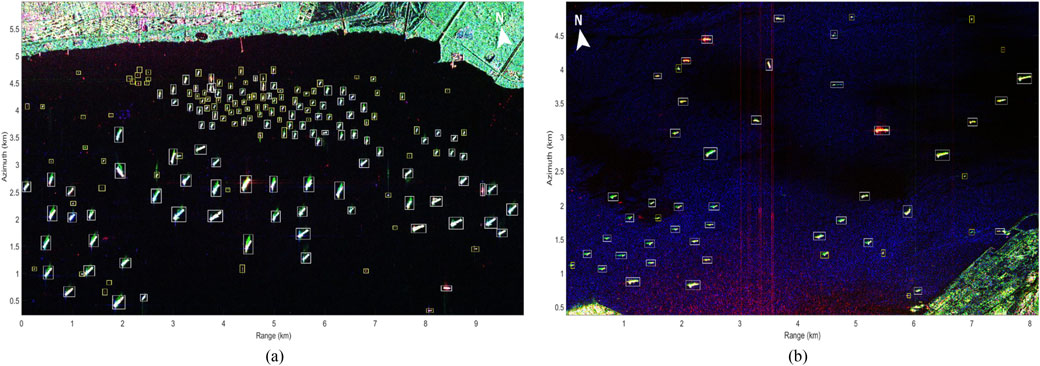
\includegraphics[width=0.97\textwidth]{appendSAR.jpg}
    \caption{RADASAT-2极化SAR图像(a)新加坡海峡(b)大连港}
    \label{fig:append:SARImage}
  \end{figure}

\subsection{参数设置}
由于变分贝叶斯推断有可能会找到局部最优解,因此必须对算法\ref{alg:append:VBI}进行适当的初始化。在下文中,我们详细
介绍了该方法潜变量的初始化和超参数设置。

1)初始化潜变量:我们采用一种简单的方法来初始化潜变量。首先我们对$\bf{D}$中所有的像素的SPAN值做升序排序。然后我们将前85\%有较低SPAN值的像素作为海杂波像素,其他有更高SPAN值的像素作为舰船像素。
因此我们获得了粗略的检测结果,其被用于初始化$\bf{A_0}$。

粗略检测得到的杂波像素值用于估计混合高斯分布的参数,其被用来初始化与海杂波$\bf{C}$相关的潜变量。我们使用贝叶斯信息准则选择混合高斯分布的分量数K。在我们实验中,我们
发现五分量的混合多元高斯分布具有足够的灵活性以适合海杂波的分布。每个${\bf{u}}_k^0,M_{k::}^0,\pi _k^0$都使用粗略检测的杂波像素来初始化。每个$z_{ij}^0$被初始化为随机的K维指示向量。
每个${\phi _k}$设置为不小于2d-1的数字,这里我们设置${\phi _k}$为6。

对于迭代停止条件,我们发现两次连续的$\bf{A}*\bf{D}$估计值之间的相对变化在五次迭代后总是小于$10^{-4}$。因此我们设置$thres=10^{-4}$,或简单的设置最大迭代次数M=10。在以下实验中我们采用后者。

2)超参数设置:以非信息的方式设置算法\ref{alg:append:VBI}中的所有超参数,以减少他们对后验分布估计的影响。因此
$\beta_1,\beta_2,{\eta_{0k}}$均被设置为$10^{-6}$。对于稀疏相关的超参数$\alpha_0$设置为$10^{-3}$,并设置$\beta_0=1-\alpha_0$。
\subsection{定义真值}
通常,从船舶自动识别系统AIS收集的数据用于最终确认舰船检测结果中虚警和漏报的船只。不幸的是我们没有与图\ref{fig:append:SARImage}相关的AIS数据。
实际上,虚警的目标通常是由较强散射的方位向模糊导致的。尤其是对于海岸附近的海域,沿海岸分布的基础设施通常会产生虚警。为了获得不含歧义的真实值,我们采用了文献[28]提出的方法,原理是校准后的
SLC图像HV与VH分量之间的相位差约为$\pi$,其幅值近似相等。因此我们可以简单的使用交叉极化SLC分量HV+VH的总和消除这种歧义。对于图\ref{fig:append:SARImage}中HV+VH强度图像如图\ref{fig:append:SARHVVHImage}所示。我们可以看到
所有因方位向模糊导致的虚警目标都被消除了。此外我们进一步使用跨度和极化信息来帮助验证反向散射强度较弱的船舶。

最终标有方框的船舶真值如图\ref{fig:append:SARImage}与图\ref{fig:append:SARHVVHImage}所示。对于新加坡海峡地区,有184艘确认的船只,长度约为25-360m。对于大连港海域
有51艘船,长度约为35-270m。在每个图像中,船只真值被换分为大船组(B组)与小船组(S组),分别用白框和黄框标记。船舶数量和相应长度列于表\ref{tab:append:SARImageGT}
  \begin{figure}[H] % use float package if you want it here
    \centering
    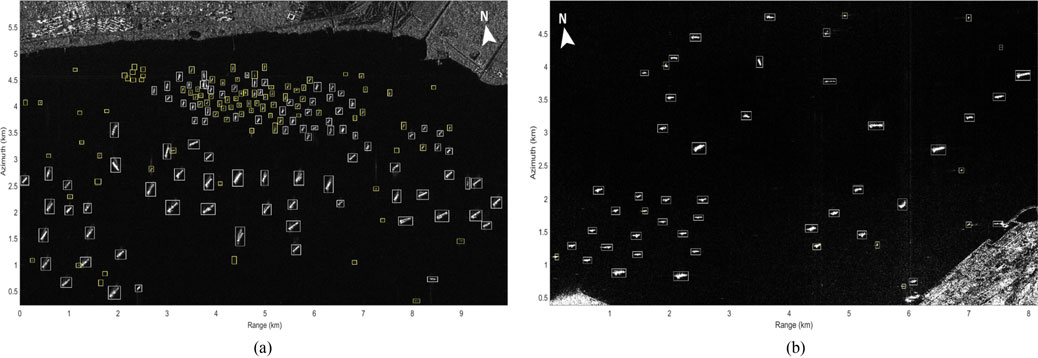
\includegraphics[width=1\textwidth]{appendSARHVVH.jpg}
    \caption{RADASAT-2${\left| {{\rm{HV}} + VH} \right|^2}$图像(a)新加坡海峡(b)大连港}
    \label{fig:append:SARHVVHImage}
  \end{figure}

  \begin{table}[htb]
  \centering
    \begin{minipage}[t]{1\linewidth} % 如果想在表格中使用脚注,minipage是个不错的办法
    \caption[船只真值]{船只真值}
    \label{tab:append:SARImageGT}
      \begin{tabularx}{\linewidth}{lXXX}
        \toprule[1.5pt]
        {\heiti 位置} & {\heiti 分组} & {\heiti 数量} &{长度(m)} \\ \midrule[1pt]
        新加坡海峡 & group B & 94 & 约125-360\\
        & group S & 90 & 约25-125\\ \midrule[1pt]
        大连港 &  group B & 40 & 约25-125 \\
        & group S & 11 & 约35-125\\
        \bottomrule[1.5pt]
      \end{tabularx}
    \end{minipage}
  \end{table}
\subsection{检测结果}
首先将遮罩应用于正在处理的图像,一种常见的陆地遮罩的方法是将SAR图像与现有的地图配准。在实验中我们手动遮盖了陆地区域。尽管这种人工
遮罩的方法并不精确,但是它不会影响舰船检测性能评估。

参考方法GP-PNF与ICS-GSD实际上是CFAR方法。在GP-PNF方法中,我们对杂波分布采用奈曼皮尔逊准则检验。GN-PNF的参数设置如下:
RedR设置便于求解数值积分的值。在这里,对于新加坡海峡与大连港,RedR分别被设置为0.1和0.01。BoxCar滤波器的最小于最大窗口尺寸
分别为$11\times 11$与$51 \times 51$。虚警率$p_{fa}$为$10^{-6}$。滑动窗的目标区域,保护区域和背景区域分别为$3\times 3$、$73\times 73$、
$93\times 93$。ICS-GSD主要使用交叉极化通道而不是所有的极化通道。在我们实验中我们将ICS-GSD应用于HV极化图像。将基于Gamma分布的
GSD用于初始检测器,然后使用迭代检测方法。GSD中虚警率设置为$10^{-8}$。此外由于海域交叉极化图像是匀质的,因此GSD无需使用滑动窗而是直接应用于
整个SAR图像。

为了定量评估检测性能,我们采用检测概率$P_d$与品质因数FoM。
\begin{equation}
    \label{equ:append:resultevaluate}
    {P_d} = \frac{{{N_d}}}{{{N_g}}},FoM = \frac{{{N_d}}}{{{N_f} + {N_g}}}
\end{equation}
其中$N_g$为船只的真值数量,$N_f$为虚警船只数量,$N_d$为正确检测的船只数量。

表\ref{tab:append:SARImageresult}和图\ref{fig:append:resultp}-图\ref{fig:append:resultr2}为使用本文方法与参考方法得到的舰船检测结果。在表\ref{}中,$N_d = N_d^B+ N_d^S$其中
$N_d^B$与$N_d^S$定义了B组和S组中船只检测数量。需要注意的是大多数由方位向模糊引起的虚警已经通过HV+VH消除。
  \begin{table}[htb]
  \centering
    \begin{minipage}[t]{1\linewidth} % 如果想在表格中使用脚注,minipage是个不错的办法
    \caption[舰船检测结果]{舰船检测结果}
    \label{tab:append:SARImageresult}
      \begin{tabularx}{\linewidth}{lXXXXX}
        \toprule[1.5pt]
        {\heiti 位置} & {\heiti 方法} & {\heiti $(N_d^B,N_d^S)$} &{\heiti $(N_d,N_f)$} &{\heiti $P_d(\%)$} &{\heiti $FoM(\%)$}\\ \midrule[1pt]
        & Proposed & (94,88) & (182,3) & 98.9 & 97.3\\
        新加坡海峡 & GP-PNF & (94,73) & (167,6) & 90.8 & 87.9\\
        & ICS-GSD & (94,80) & (174,3) & 94.6 & 93.0\\ \midrule[1pt]
        & Proposed & (40,11) & (51,0) & 100 & 100\\
        大连港& GP-PNF & (40,8) & (48,0) & 94.1 & 94.1\\
        & ICS-GSD & (40,11) & (51,2) & 100& 96.2\\
        \bottomrule[1.5pt]
      \end{tabularx}
    \end{minipage}
  \end{table}
1)比较检测结果的$P_d$与$FoM$,在图\ref{fig:append:resultp}所示的新加坡海峡区域,我们可以看到我们提出的方法可以检测到B组中所有94艘大船与S组90艘小船中的88艘,其中三艘为虚警。
对于大连港区域,我们的方法可以检测出B组所有50艘大船与S中所有11艘小船,没有虚警船只,因此我们提出的方法对于新加坡海峡图像的$P_d$为$98.9\%$,FoM为$97.3\%$。
对于大连港海域$P_d$与FoM均为$100\%$。

另一方面,对于新加坡海峡区域,GP-PNF检测器检测出了B组中所有94艘大型船舶,但仅检测出S组中的73艘小型船舶与六个虚警船只。对于大连港区域
,GP-PNF检测器检测出了B组所有40艘大型船只和S组8艘小型船只没有虚警船只。因此对于新加坡海峡区域,GP-PNF检测器的$P_d$与FoM分别为$90.8\%$与$87.9\%$,
相较于我们提出的方法分别低了$8.1\%$和$9.4\%$。对于大连港区域,GP-PNF检测器的$p_d$与FoM均为$94.1\%$,比我们提出的方法低$5.9\%$。

ICS-GSD检测器的性能优于GP-PNF,但没有我们提出的方法好。对于新加坡海峡区域,ICS-GSD检测器检测到了B组中所有的94艘大船,S组中80艘小船与三艘虚警。
对于大连港区域,ICS-GSD检测器检测到了B组40艘大船与S组11艘小船与两艘虚警。因此ICS-GSD检测器$P_d$与FoM分别为$94.6\%$和$93.0\%$,分别比本文方法低$4.3\%$。
对于大连港区域,ICS-GSD检测器的$P_d$和FoM分别为$100\%$和$96.2\%$,与本文方法的$P_d$相同,FoM稍差些。这些统计结果列于表\ref{tab:append:SARImageresult}。

简而言之,参考$P_d$和FoM的结果,本文提出的方法比参考方法具有更好的性能。

2)检测结果的形状比较:通过比较图\ref{fig:append:resultp}-\ref{fig:append:resultr2}的结果,我们可以看出,我们提出的方法和ICS-GSD检测器捕获了船舶上的主要散射。
然而,GP-PNF检测器往往会将舰船周围受影响的海杂波像素检测出来。换言之,本文方法和ICS-GSD检测器具有比GP-PNF检测器更好的形状保持能力。在此形状是指传播上
散布物的分布结构。本文方法具有较好形状保持能力的原因是特殊的变分贝叶斯推断过程。估计每个像素对应的潜变量实际上用到了其他所有的像素。因此判断每个像素的属性(舰船或杂波)时
隐式的考虑了整张图像的所有像素。因此,相比于基于滑动窗使用有限样本的方法本文方法具有更好的检测结果是合理的。ICS-GSD检测器的形状保持能力源于迭代检查方案。对于GP-PNF检测器,应
使用滑动窗获得一些参数。这些平均的操作可能会使舰船模糊,甚至会擦除一些小型船只。因此就形状保持能力而言,本文方法和ICS-GSD方法的性能优于GP-PNF方法。

3)与单通道检测器进行比较:在文献[20]中,变分贝叶斯推断方法被首次应用于单通道SAR图像舰船检测。详细来讲从新加坡海峡获得的HH通道图像被应用于实验测试。
检测结果的$P_d$与FoM值为$88.6\%$与$86.2\%$,比本文方法差
  \begin{figure}[H] % use float package if you want it here
    \centering
    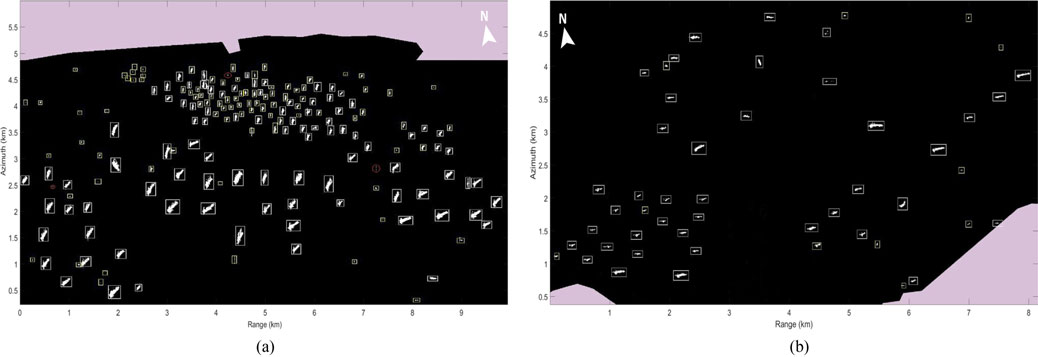
\includegraphics[width=1\textwidth]{appendresult.jpg}
    \caption{本文提出方法检测结果(a)新加坡海峡(b)大连港}
    \label{fig:append:resultp}
  \end{figure}
  \begin{figure}[H] % use float package if you want it here
    \centering
    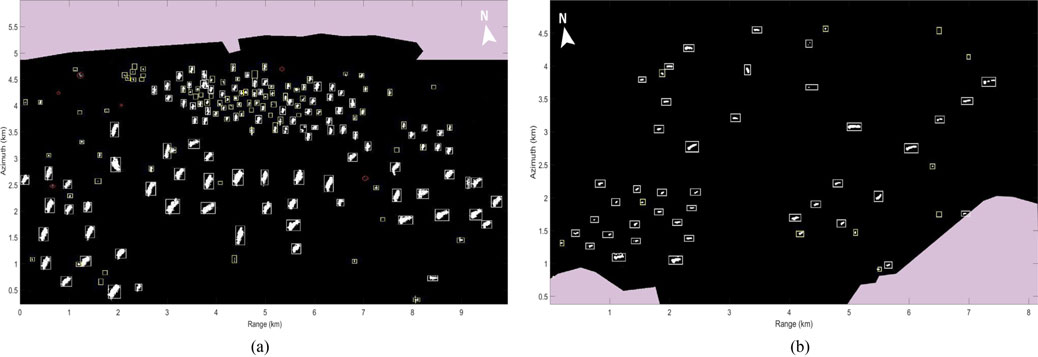
\includegraphics[width=1\textwidth]{appendr1result.jpg}
    \caption{GP-PNF检测结果(a)新加坡海峡(b)大连港}
    \label{fig:append:resultr1}
  \end{figure}
  \begin{figure}[H] % use float package if you want it here
    \centering
    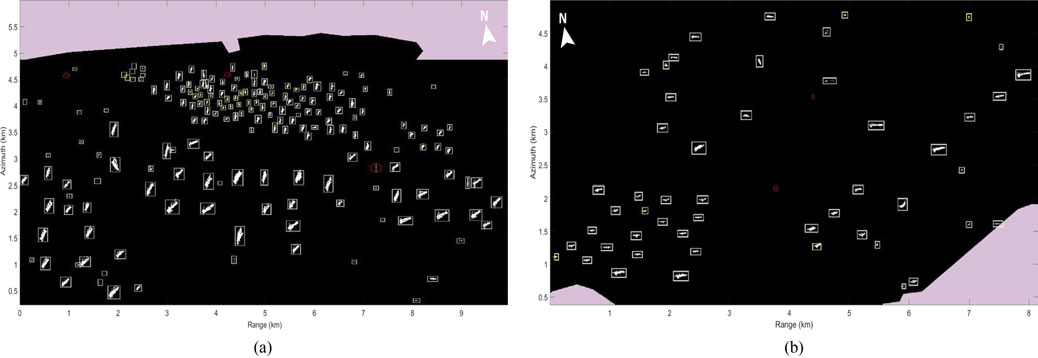
\includegraphics[width=1\textwidth]{appendr2result.jpg}
    \caption{ICS-GSD检测结果(a)新加坡海峡(b)大连港}
    \label{fig:append:resultr2}
  \end{figure}
\noindent 很多。因此我们可以得出结论,极化信息确实有助于进一步提升舰船检测性能。此外通过比较本文方法与
ICS-GSD检测器的结果,我们可以看到尽管交叉极化非常适用于舰船检测,但将所有极化通道与变分贝叶斯推断结合起来比单通道检测器方法具有更好的性能。

4)时间消耗,本文方法和参照方法均以MATLAB代码编写,所有的实验均在MATLAB软件上进行,使用的工作站配有Intel Core i7处理器频率为3.4GHZ,内存为8G。
不同方法时间消耗列于表\ref{tab:append:SARresultTime}。我们可以看到本文方法比GP-PNF方法快,但比ICS-GSD方法慢很多。主要原因取决于
算法\ref{alg:append:VBI}的特殊程序结构,其中更新潜变量的的期望值是高度耦合的并依赖所有的极化通道。ICS-GSD算法效率非常高是因为
GSD初始检测器应用于整个交叉极化图像而非滑动窗,以及采用简单的杂波分布Gamma分布。而且ICS-GSD检测磁通常不需要两次以上的迭代就能够达到收敛。
GP-PNF检测器使用滑动窗,并且通过计算数值积分获得每个像素的阈值,因此非常耗时。

简而言之,虽然本文方法在速度上差强人意,但是它具有更高的$F_d$、FoM与良好的形状保持能力。特别是如图\ref{fig:append:SARImage}(a)所示的拥挤海域,本文的方法比参考方法
有更多的优势。

  \begin{table}[htb]
  \centering
    \begin{minipage}[t]{1\linewidth} % 如果想在表格中使用脚注,minipage是个不错的办法
    \caption[不同方法时间消耗]{不同方法时间消耗}
    \label{tab:append:SARresultTime}
      \begin{tabularx}{\linewidth}{lXX}
        \toprule[1.5pt]
        {\heiti 位置} & {\heiti 方法} & {\heiti 时间} \\ \midrule[1pt]
        & 本文方法 & 12.9min \\
        新加坡海峡 & GP-PNF & 158.3min\\
        & ICS-GSD & 7.6s\\ \midrule[1pt]
        & 本文方法 & 8.2min \\
        大连港 &  GP-PNF & 184.8min \\
        & ICS-GSD & 4.6s \\
        \bottomrule[1.5pt]
      \end{tabularx}
    \end{minipage}
  \end{table}
\section{结论}
本文提出了一种创新的极化SAR图像舰船检测方法。我们首先将极化SAR图像分解为稀疏的船舶分量和海杂波分量,并引入与这些分量相关的潜变量
的层次先验,从而建立了极化SAR图像舰船检测的概率模型。然后采用变分贝叶斯推断方法来估计潜变量的期望值,从变分贝叶斯迭代推理过程获得获得最终的
检测结果。

我们已使用C波段RADARSAT-2极化SAR图像来评估方法的有效性。最新的GP-PNF检测器与ICS-GSD检测器作为参考方法。结果表明本文提出方法在
$P_d$、FoM与形状保持能力方面优于参考方法。本分方法良好的检测性能源于两个因素,第一个是显示的使用了所有
极化通道不需要极化信息融合。第二个是特殊的变分贝叶斯推断原理,这种方法不需要使用滑动窗。尽管本文提出的方法时间性能上略差一些,
但是它具有良好的适应性,尤其是对于一些具有挑战性的应用场景如拥挤海域。

未来的工作将集中在以下两个方面。首先应提高本文方法的时间效率,借助于程序优化与并行计算技术,我们可以进一步加速程序。第二可以利用舰船像素
之间的依赖性去进一步提升算法的形状保持能力。

